%TITULO-------------------------------------------------------------------

%=========================================================================
\chapter{Resultados}\label{resultados}
%=========================================================================

  A comprovação da teoria desenvolvida nos capítulos anteriores é feita através da demonstração de resultados de simulação e experimentais. As simulações são feitas utilizando o software \textsc{Matlab}, da empresa \textit{MathWorks}$^\circledR$. Mais especificamente, o \textit{toolbox} Simulink é o componente central para realização das simulações. O filtro \textit{LCL} é descrito como uma função de transferência conforme o Capítulo~\ref{modelagem}, o conversor e a fonte são simulados usando modelos disponíveis no Simulink. A plataforma \textsc{dSpace} serve como uma interface entre o circuito real e o \textsc{Matlab}, dispondo de $n_{ADs}$ conversores analógico-digitais (\emph{AD}) de $n$ bits e $n_{DAs}$ conversores digitais-analógicos (\emph{DA}) de $n$ bits, através dos quais são adquiridas as medidas feitas em tempo real no circuito. A plataforma se encarrega de disponibilizar as medidas adquiridas em um bloco do Simulink, permitindo que sejam utilizadas diretamente no cálculo da ação de controle. Uma vez computada, a ação de controle é transcrita em comando de acionamento das chaves do conversor e então enviada via \emph{DA} para o conversor.

  Os resultados experimentais são obtidos utilizando uma bancada composta por uma fonte \textit{modelo}, um conversor \textsc{Semikron} \textit{modelo} com $n V$ de tensão e $n A$ de corrente nominais. A interface \textsc{dSpace} utilizada é o modelo \textit{modelo}. O processador que a unidade possui é um \emph{DSP} - do inglês \emph{Digital Signal Processor} modelo $modelo$ com uma unidade de lógica e aritmética de ponto flutuante de $n$ bits. As medidas da tensão e corrente do capacitor, bem como da corrente do lado da rede foram feitas utilizando sensores de Efeito Hall. A ação de controle é modulada por largura de pulso e enviada para o \emph{DSP} via um bloco específico da plataforma no \emph{Simulink}. A Fig.~\ref{fig:topologia_bancada} apresenta a disposição dos elementos da bancada.

  \begin{figure}[htb]
    \centering{
      %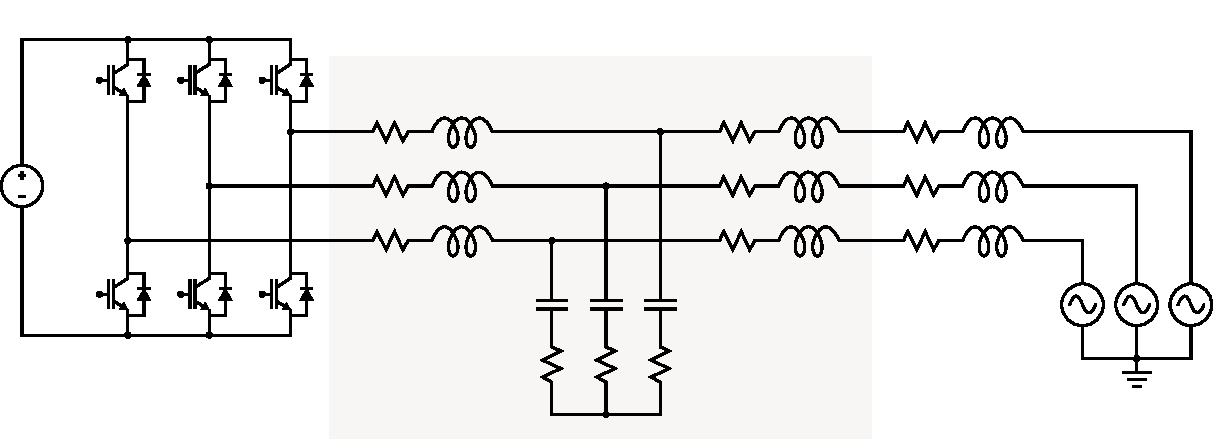
\includegraphics[width=0.9\textwidth]{img/topologia}}
      \def\svgwidth{0.9\textwidth}
      \input{./img/bancada.pdf_tex}}
    \renewcommand\figurename{Fig.}
    \caption{Diagrama que representa os elementos da bancada.}
    \label{fig:topologia_bancada}
  \end{figure}


\section{Resultados de Simulação}

	%figura mostrando o sistema
  %que tipo de conversor é, que marca, que modelo, dados nominais
  %que tipos de sensores foram usados? como foram feitas as medidas?
  %que tipo de controlador digital foi usado? modelo do dsp na dspace
  %quantos bits têm os conversores a/d?
  %como é acionado o conversor?
  %qual a frequência de amostragem? e a de comutação?
  %colocar numa tabela: tensão de linha, frequência, tensão do barramento cc, indutâncias e capacitância do filtro, frequência de amostragem e de comutação
  %comentar que os resultados obtidos foram para o equivalente monofásico
  %apresentar expressão do modelo de referência
  %apresentar expressões dos vetores w
  %apresentar os valores iniciais dos ganhos do controlador adaptativo (kp, gamma, rho, etc)
  %apresentar os valores de inicialização dos thetas
  %comentar sobre o sinal de normalização m^2

  O Simulink dispõe de muitos blocos cujos modelos matemáticos são geralmente aceitos como precisos o suficiente para representar elementos do mundo real. Por isso, os modelos de conversor, linha de transmissão, transformador e fonte são utilizados neste trabalho para representar o comportamento de elementos reais.

	A ação de controle é implementada na simulação via código escrito em linguagem própria do \textsc{Matlab}, chamada \textit{linguagem .m}. Existe um bloco no Simulink chamado \textit{Subsystem}, que recebe sinais de entrada e permite que esses sinais sejam manipulados via código para gerarem sinais de saída. Este bloco é utilizado para implementar a ação de controle projetada nos capítulos anteriores.

	Como a simulação é implementada em tempo discreto, os principais passos realizados são os seguintes:

	\begin{enumerate}
		\item \textit{Inicialização}: no início da simulação, são carregados os valores iniciais para as variáveis;
		\item \textit{Amostragem das variáveis}: as variáveis são amostradas para a realização dos cálculos preliminares da ação de controle;
    \item \textit{Conversão de coordenadas $abc$ para $\alpha \beta 0$}: é aplicada a transformação de desacoplamento nas variáveis;
		\item \textit{Cálculo da ação de controle}: a ação de controle é calculada e o estado atual das variáveis é armazenado como sendo o estado anterior para a próxima iteração da simulação;
    \item \textit{Acionamento do conversor}: a ação de controle é modulada por largura de pulso e as chaves do conversor são acionadas;
		\item \textit{Geração da saída}: são feitas as medidas da corrente e tensão do capacitor, e da corrente do lado da rede.
	\end{enumerate}

  O projeto do controlador é conforme o Capítulo~\ref{controle}. O modelo de referência projetado é da forma
  %
  \begin{equation}
    W_m(z) = \frac{(1-p_1)(1-p_2)}{(z-p_1)(z-p_2)}\text{,}
    \label{eq:wm_simulacao}
  \end{equation}
  %
  com $p_1 = p_2 = 0,2$.

	A Tabela~\ref{tab:parametros_projeto} resume os demais parâmetros utilizados no projeto. Os valores de inicialização dos parâmetros são baseadas nos valores ideais, ou seja, aqueles que fazem com que os valores dos ganhos adaptativos $\theta$ sejam $\theta^*$ (valores para a condição de casamento). Os valores de inicialização dos ganhos adaptativos, neste caso, são dados por \ref{eq:theta_ini}.
  %
  \begin{equation}
    \begin{split}
      \theta^T & = \left[ \begin{matrix} -0,03, & -0,36, & -0,57, & -0,01 & 0,16 & 0,02 \end{matrix} \right]\text{ e}\\
      \omega & = {\left[ \begin{matrix} 0 & 0 & 0 & 0 & 0 & 0 \end{matrix} \right]}^T\text{.}
    \end{split}
    \label{eq:theta_ini}
  \end{equation}

  \begin{table}[htb]
    \renewcommand{\arraystretch}{1.35}
    \setlength{\tabcolsep}{1.2mm}
    \caption{Valores dos parâmetros do sistema utilizados no projeto.}
    \label{tab:parametros_projeto}
    \centering
    \begin{tabular}{l l l l}
      \hline
      \multicolumn{1}{c}{Parâmetro} & \multicolumn{1}{c}{Valor} &
      \multicolumn{1}{c}{Parâmetro} & \multicolumn{1}{c}{Valor} \\
      \hline
      $L_1$      & $2$mH    & $L_2$         & $2$mH  \\
      $C$        & $40\mu$F & $f_s = 1/T_s$ & $12$kHz\\
      $\gamma_d$ & $0,0098$ & $\gamma$      & $0,99$ \\
      $\delta_0$ & $0,8$    &               & \\
      \hline
    \end{tabular}
  \end{table}

  %separar em três figuras, uma pra inversão de fase, outra pra degrau de amplitude e outra pra variação da indutância
  A Fig.~\ref{fig:i2_simulacao_inv_fase} apresenta a corrente da rede em comparação com a referência. No instante $t_1 = \pi s$ ocorre inversão de fase na referência. A Fig.~\ref{fig:i2_simulacao_degrau} apresenta, no instante $t_2$, um degrau de amplitude aplicado à referência. Na Fig.~\ref{fig:i2_simulacao_L_rede} apresenta uma variação na indutância da rede no instante $t_3$.

	\begin{figure}[htb]
    \centering
      \def\svgwidth{0.8\textwidth}
      \input{./img/logo.pdf_tex}
    \renewcommand\figurename{Fig.}
    \caption{Inversão de fases na referência.}
    \label{fig:i2_simulacao_inv_fase}
  \end{figure}

  \begin{figure}[htb]
    \centering
      \def\svgwidth{0.8\textwidth}
      \input{./img/logo.pdf_tex}
    \renewcommand\figurename{Fig.}
    \caption{Degrau de amplitude na referência.}
    \label{fig:i2_simulacao_degrau}
  \end{figure}

  \begin{figure}[htb]
    \centering
      \def\svgwidth{0.8\textwidth}
      \input{./img/logo.pdf_tex}
    \renewcommand\figurename{Fig.}
    \caption{Variação da indutância da rede.}
    \label{fig:i2_simulacao_L_rede}
  \end{figure}

  %incluir figura mostrando a convergência dos thetas
  %incluir figura mostrando a parcela do vetor w referente a rejeição do distúrbio de tensão da rede

\section{Resultados Experimentais}



%FIM----------------------------------------------------------------------
